\documentclass[a4paper, 14pt]{extarticle}
\usepackage[settings]{markdown}
\usepackage{minted}

% Поля
%--------------------------------------
\usepackage{geometry}
\geometry{a4paper,tmargin=2cm,bmargin=2cm,lmargin=3cm,rmargin=1cm}
%--------------------------------------


%Russian-specific packages
%--------------------------------------
\usepackage[T2A]{fontenc}
\usepackage[utf8]{inputenc} 
\usepackage[english, main=russian]{babel}
%--------------------------------------

\usepackage{textcomp}

% Красная строка
%--------------------------------------
\usepackage{indentfirst}               
%--------------------------------------             


%Graphics
%--------------------------------------
\usepackage{graphicx}
\graphicspath{ {./images/} }
\usepackage{wrapfig}
%--------------------------------------

% Полуторный интервал
%--------------------------------------
\linespread{1.3}                    
%--------------------------------------

%Выравнивание и переносы
%--------------------------------------
% Избавляемся от переполнений
\sloppy
% Запрещаем разрыв страницы после первой строки абзаца
\clubpenalty=10000
% Запрещаем разрыв страницы после последней строки абзаца
\widowpenalty=10000
%--------------------------------------

%Списки
\usepackage{enumitem}

%Подписи
\usepackage{caption} 

%Гиперссылки
\usepackage{hyperref}

\hypersetup {
	unicode=true
}

%Рисунки
%--------------------------------------
\DeclareCaptionLabelSeparator*{emdash}{~--- }
\captionsetup[figure]{labelsep=emdash,font=onehalfspacing,position=bottom}
%--------------------------------------

\usepackage{tempora}
\usepackage{amsmath}
\usepackage{color}
\usepackage{listings}
\lstset{
  belowcaptionskip=1\baselineskip,
  breaklines=true,
  frame=L,
  xleftmargin=\parindent,
  language=Python,
  showstringspaces=false,
  basicstyle=\footnotesize\ttfamily,
  keywordstyle=\bfseries\color{blue},
  commentstyle=\itshape\color{purple},
  identifierstyle=\color{black},
  stringstyle=\color{red},
}

%--------------------------------------
%			НАЧАЛО ДОКУМЕНТА
%--------------------------------------

\begin{document}

%--------------------------------------
%			ТИТУЛЬНЫЙ ЛИСТ
%--------------------------------------
\begin{titlepage}
\thispagestyle{empty}
\newpage


%Шапка титульного листа
%--------------------------------------
\vspace*{-60pt}
\hspace{-65pt}
\begin{minipage}{0.3\textwidth}
\hspace*{-20pt}\centering

\includegraphics[width=\textwidth]{emblem}
\end{minipage}
\begin{minipage}{0.67\textwidth}\small \textbf{
\vspace*{-0.7ex}
\hspace*{-6pt}\centerline{Министерство науки и высшего образования Российской Федерации}
\vspace*{-0.7ex}
\centerline{Федеральное государственное бюджетное образовательное учреждение }
\vspace*{-0.7ex}
\centerline{высшего образования}
\vspace*{-0.7ex}
\centerline{<<Московский государственный технический университет}
\vspace*{-0.7ex}
\centerline{имени Н.Э. Баумана}
\vspace*{-0.7ex}
\centerline{(национальный исследовательский университет)>>}
\vspace*{-0.7ex}
\centerline{(МГТУ им. Н.Э. Баумана)}}
\end{minipage}
%--------------------------------------

%Полосы
%--------------------------------------
\vspace{-25pt}
\hspace{-35pt}\rule{\textwidth}{2.3pt}

\vspace*{-20.3pt}
\hspace{-35pt}\rule{\textwidth}{0.4pt}
%--------------------------------------

\vspace{1.5ex}
\hspace{-35pt} \noindent \small ФАКУЛЬТЕТ\hspace{50pt} <<Информатика и системы управления>>

\vspace*{-16pt}
\hspace{47pt}\rule{0.83\textwidth}{0.4pt}

\vspace{0.5ex}
\hspace{-35pt} \noindent \small КАФЕДРА\hspace{50pt} <<Теоретическая информатика и компьютерные технологии>>

\vspace*{-16pt}
\hspace{30pt}\rule{0.866\textwidth}{0.4pt}
  
\vspace{11em}

\begin{center}
\Large {\bf Лабораторная работа № 4} \\ 
\large {\bf по курсу <<Базы данных>>}\\
\end{center}\normalsize

\vspace{8em}


\begin{flushright}
  {Студент группы ИУ9-51Б Горбунов А. Д.\hspace*{15pt} \\
  \vspace{2ex}
  Преподаватель Вишняков И. Э.\hspace*{15pt}}
\end{flushright}

\bigskip

\vfill
 

\begin{center}
\textsl{Москва 2024}
\end{center}
\end{titlepage}
%--------------------------------------
%		КОНЕЦ ТИТУЛЬНОГО ЛИСТА
%--------------------------------------

\renewcommand{\ttdefault}{pcr}

\setlength{\tabcolsep}{3pt}
\newpage
\setcounter{page}{2}

\section{Задача}\label{Sect::task}
\par

\begin{enumerate}
    \item Преобразовать модель семантических объектов, созданную в лабораторной работе №2, в реляционную модель согласно процедуре преобразования.
    \item Сопоставить результаты проектирования с использованием модели «сущность-связь» и модели семантических объектов (лабораторные работы №3,4).
    \item Обосновать различия результатов, выявить и исправить ошибки проектирования.
\end{enumerate}

\par

\section{Практическая реализация}\label{Sect::task}
    На рисунке 1 представлена созданная в лабораторной работе №2 модель семантических объектов:

\begin{figure}[!htb]
	\centering
	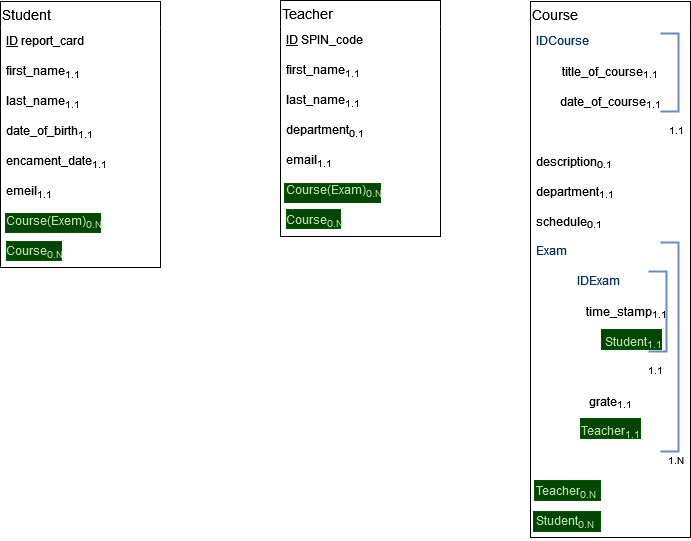
\includegraphics[width=0.8\textwidth]{scheme_lab_2.png}
\caption{Модель семантических объектов}
\label{fig:scheme}
\end{figure}

    В соответствии с правилами преобразования, из созданной ранее семантической модели, получили реляционную модель, представленную на рисунке 2:

\begin{figure}[!htb]
	\centering
	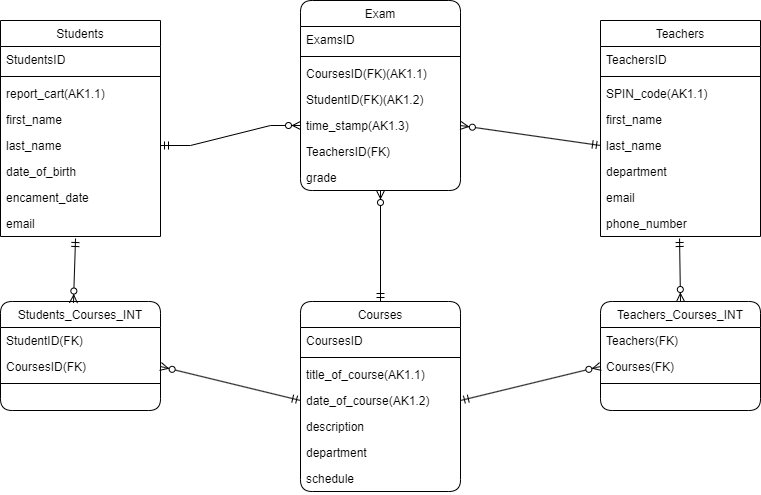
\includegraphics[width=0.8\textwidth]{scheme.png}
\caption{Реляционная модель, полученная из модели семантических объектов}
\label{fig:scheme}
\end{figure}

    Модель, полученная в 3 лабораторной работе, представлена на рисунке 3:

\begin{figure}[!htb]
	\centering
	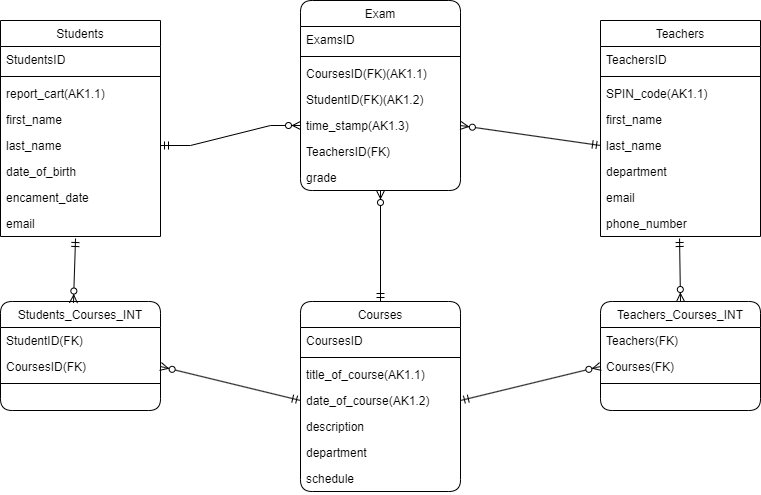
\includegraphics[width=0.8\textwidth]{scheme_lab_3.png}
\caption{Реляционная модель, полученная из модели «сущность-связь»}
\label{fig:scheme}
\end{figure}

    Реляционные модели, полученные из разных моделей данных, получились абсолютно идентичные. Кроме различия, что в лабораторной №4 были выбраны дополнительно альтернативные ключи.

\end{document}
